\documentclass[12pt]{article}
\usepackage{graphicx} % Required for inserting images
\usepackage{amsmath,amssymb,amsthm,amsfonts}
\usepackage{xcolor}
\usepackage{tasks}
%\usepackage{enumitem}
\usepackage[margin=2cm]{geometry}
\usepackage{tkz-euclide}

\usepackage[utf8]{inputenc}
\usepackage[T1]{fontenc}
\usepackage{amsmath}
\usepackage{amsfonts}
\usepackage{amssymb}
\usepackage[version=4]{mhchem}
\usepackage{stmaryrd}
\usepackage{enumerate}
\usepackage{multicol}
\usepackage{xcolor}
\usepackage{graphicx}
\usepackage{ulem}
\usepackage{cancel}
\usepackage{tikz}
\usepackage{tkz-euclide}
\usepackage[finnish]{babel}

%\usepackage[style=alphabetic,]{biblatex}

%\usepackage[margin=2cm]{geometry}

\newcommand{\brac}[1]{\left(#1\right)}
\newcommand{\sqbrac}[1]{\left[#1\right]}
\newcommand{\set}[1]{\left\{#1\right\}}

\newcommand{\dd}[0]{\mathrm{d}}
\newcommand{\dx}[0]{\mathrm{d}x}

\newcommand{\hatu}{\hat{u}}
\newcommand{\hatv}{\hat{v}}
\newcommand{\hatw}{\hat{w}}
\newcommand{\hatn}{\hat{n}}

\newcommand{\vu}{\overline{u}}
\newcommand{\vv}{\overline{v}}
\newcommand{\vw}{\overline{w}}
\newcommand{\vp}{\overline{p}}
\newcommand{\vn}{\overline{n}}

\newcommand{\va}{\overline{a}}
\newcommand{\vb}{\overline{b}}
\newcommand{\vc}{\overline{c}}
\newcommand{\vd}{\overline{d}}


\newcommand{\vi}{\hat{\imath}}
\newcommand{\vj}{\hat{\jmath}}
\newcommand{\vk}{\hat{k}}

\newcommand{\ratkaisu}[1]{\hfill{\color{blue}\quad\textrm{Ratkaisu: } #1}}

\newcommand{\ratkaisuu}[1]{{\color{blue}\textrm{Ratkaisu: } #1}}

\newcommand{\kaava}[1]{{\color{green!50!black}#1}}

%\renewcommand{\ratkaisu}[1]{}
%\renewcommand{\ratkaisuu}[1]{}
%\renewcommand{\kaava}[1]{}

\newcommand{\vihje}[1]{{\color{red}Vihje. #1}}
\newcommand{\extra}[0]{\textbf{Extra.}~}

\title{OAMK}
\author{Juha-Matti Huusko}
\date{August 2023}

\renewcommand{\ratkaisu}[1]{{\color{blue}\quad\textrm{Ratkaisu: } #1}}

\renewcommand{\ratkaisu}[1]{}

\begin{document}
\thispagestyle{empty}

\section*{Läpipääsytentti 26.3.2024}
\subsubsection*{Matematiikan perusteet tietotekniikassa 2, IN00EH21-3001}

\begin{enumerate}
\item Laske funktion $f(x)=4\sin(x)-\cos(2x)$ keskimääräinen muutosnopeus välillä $[0,2]$.
\item Laske $f'(x)$, kun
\begin{enumerate}
\item $f(x)=4x^5-\sqrt{2x}+\frac{1}{x^3}$
\item $f(x)=2\sin(3x)-7e^{x^4}$
\item $f(x)=e^x\ln(x)$
\end{enumerate}
\begin{figure}[h!]
    \centering
\def\px{1}
\def\py{2}
\def\qx{4}
\def\qy{3}
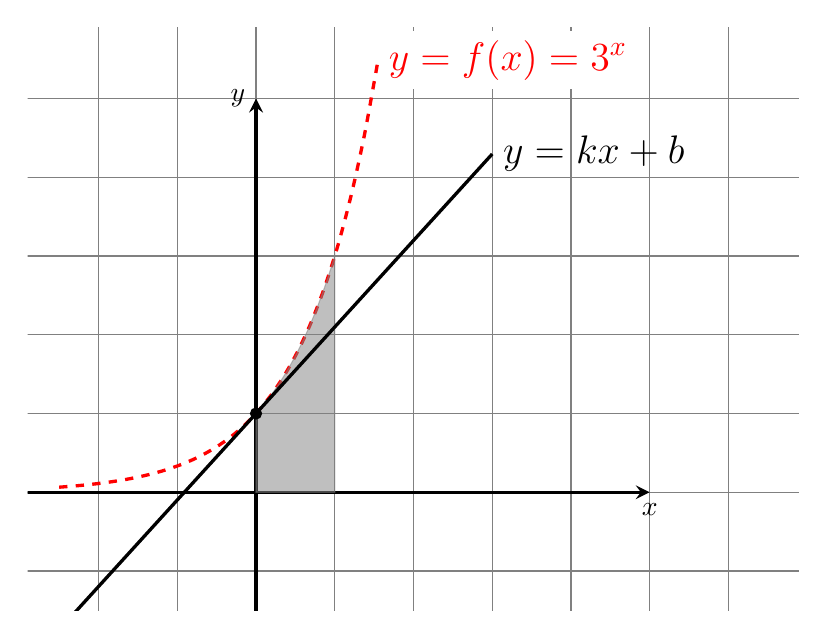
\begin{tikzpicture}[>=stealth]
\path[clip] (-2.9,-1.5) rectangle (6.9,5.9);
\draw[gray] (-6.9,-6.9) grid (6.9, 6.9);
\draw[very thick,->] (-5,0)--(5,0) node[below]{$x$};
\draw[very thick,->] (0,-5)--(0,5) node[left]{$y$};
%\draw[very thick, blue, domain=-2.5:2.5,smooth,variable=\t] plot ({\t},{1+0.693*\t+0.24*\t*\t});
\draw[very thick, red, dashed, domain=-2.5:1.55,smooth,variable=\t]
  plot ({\t},{exp(1.0986*\t)}) node[fill=white,right]{{\Large $y=f(x)=3^x$}};
\filldraw[gray, opacity=0.5, domain=0:1,smooth,variable=\t]
  plot ({\t},{exp(1.0986*\t)}) -- (1,0) --(0,0)--cycle;
\draw[very thick] (-3,-2.2958)--(3,4.2958) node[right]{{\Large $y=kx+b$}};
\filldraw (0,1) circle (2pt);
\end{tikzpicture}
    \caption{Funktion kuvaaja, tangenttisuora ja pinta-ala. Ruudun leveys ja korkeus ovat 1.}
    \label{fig:eksponentti-deri-int}
\end{figure}
\item Selvitä Kuvassa~\ref{fig:eksponentti-deri-int} olevan suoran $y=kx+b$ yhtälö.
\item Selvitä Kuvassa~\ref{fig:eksponentti-deri-int} olevan varjostetun alueen pinta-ala.
\item Uima-altaan tilavuuden tulee olla 256 kuutiometriä. Altaan pohja on neliön muotoinen ja seinät pystysuorat. Suunnittele altaan mitoitus niin, että kaakelia kuluu mahdollisimman vähän, kun seinät ja pohja kaakeloidaan. Toisin sanoen minimoi seinien ja pohjan yhteenlaskettu pinta-ala.
\item Laske
\begin{enumerate}
\item $\int 4x+\sqrt{x}dx$
\item $\int \cos(2x)dx$
\item $\int_2^3 e^{-x}+1dx$
\end{enumerate}
\end{enumerate}

\section*{Kaavat (Matematiikan perusteet tietotekniikassa 2)}

$$y-y_1=k(x-x_1),\quad y=kx+b,\quad k=\frac{y_2-y_1}{x_2-x_1}=f'(x_1)$$

$$
\int_a^b f(x)dx=\bigg |_a^b F(x)=F(b)-F(a),\quad F'(x)=f(x)
$$

$$
\begin{array}{rl|rl}
\textbf{Derivointi} && \textbf{Integrointi}&\\[2mm]
Dx^n&=nx^{n-1}     \qquad\qquad&\qquad\qquad\int x^ndx&=\frac{x^{n+1}}{n+1}+C \\[2mm]
De^x&=e^x &\int e^xdx&=e^x+C\\[2mm]
Db^x&=b^x\ln(b) & \int b^xdx&=\frac{b^x}{\ln(b)}\\[2mm]
D\ln(x)&=\frac{1}{x} &&\\[2mm]
D\ln|x|&=\frac{1}{x} &\int\frac{1}{x}dx&=\ln|x|+C\\[2mm]
D\log_a(x)&=\frac{1}{x\ln(a)} &&\\[2mm]
D\log_a|x|&=\frac{1}{x\ln(a)} &&\\[2mm]
D\sin(x)&=\cos(x)   &\int\cos(x)dx&=\sin(x)+C\\[2mm]
D\cos(x)&=-\sin(x)  &\int\sin(x)dx&=-\cos(x)+C\\[2mm]
D\tan(x)&=1+\tan^2(x) \qquad&\qquad\int 1+\tan^2(x)dx&=\tan(x)+C\\[2mm]

Dx\ln(x)-x&=\ln(x) & \int\ln(x)dx&=x\ln(x)-x+C\\[10mm]

D\arcsin(x)&=\frac{1}{\sqrt{1-x^2}} & \int\frac{1}{\sqrt{1-x^2}}&=\arcsin(x)+C\\
D\arccos(x)&=\frac{1}{-\sqrt{1-x^2}} & \int\frac{1}{-\sqrt{1-x^2}}&=\arccos(x)+C\\
D\arctan(x)&=\frac{1}{1+x^2} & \int\frac{1}{1+x^2}&=\arctan(x)+C\\

D\sinh(x)&=\cosh(x) &&\\
D\cosh(x)&=\sinh(x) &&\\
D\tanh(x)&=\frac{1}{\cosh^2(x)} &&\\
\end{array}  
$$
\vspace{1cm}
$$
\begin{array}{rl|rl}
\textbf{Derivointi} && \textbf{Integrointi}&\\[2mm]
D f(g(x))&=f'(g(x))g'(x) & \int f(g(x))g'(x)dx&=f(g(x))+C\\[2mm]
\textrm{Erikoistapauksia} &&&\\
D\ln(f(x))&=\frac{f'(x)}{f(x)} & \int \frac{f'(x)}{f(x)}dx&=\ln(f(x))+C\\[2mm]
D e^{f(x)}&=e^{f(x)}f'(x) & \int f'(x)e^{f(x)}dx&=e^{f(x)}+C\\[10mm]
D fg&=f'g+fg'& \int f'g dx&=fg-\int fg'dx\\[2mm]
D (f/g)&=(gf'-fg')/g^2 &&\\[2mm]
\end{array}  
$$

\section*{Kaavat (Matematiikan perusteet tietotekniikassa 1)}

Murtoluvut
$$
\frac{a}{b}+\frac{c}{d}=\frac{ad}{bd}+\frac{bc}{bd}
=\frac{ad+bc}{bd},\quad 
\frac{a}{b}\cdot\frac{c}{d}=\frac{ac}{bd},\quad
\frac{a}{b}\bigg/\frac{c}{d}=\frac{a}{b}\cdot\frac{d}{c}=\frac{ad}{bc}
$$
Potenssit
$$
a^ba^c=a^{b+c},\quad 
\frac{a^b}{a^c}=a^{b-c},\quad 
(a^b)^c=a^{bc},\quad 
(ab)^c=a^ba^c,\quad 
\brac{\frac{a}{b}}^c=\frac{a^b}{b^c}
$$
Juuret
$$
(a^b)^{\frac{1}{b}}=a^{b\cdot \frac{1}{b}}=a^1=a,\quad\textrm{jos}\quad a>0,\quad 
\sqrt{a}=a^{\frac{1}{2}},\quad \sqrt[3]{a}=a^{\frac{1}{3}}
$$
Ensimmäisen asteen yhtälö
$$
ax=b\quad\Leftrightarrow\quad x=\frac{b}{a}
$$
Toisen asteen yhtälö
$$
ax^2+bx+c=0\quad\Leftrightarrow\quad x=\frac{-b\pm\sqrt{b^2-4ac}}{2a}
$$
Yhtälöpari
$$
\begin{cases}
ax+by&=U\\
cx+dy&=V
\end{cases}\quad\Rightarrow
\begin{cases}
acx+bcy&=cU\\
-acx+-ady&=-aV
\end{cases}\Rightarrow\ldots
$$

$$
\begin{cases}
ax+by&=U\\
cx+dy&=V
\end{cases}\quad\Rightarrow
y=\frac{U-ax}{b}\quad\Rightarrow
cx+d\frac{U-ax}{b}=V\Rightarrow\ldots
$$

$$
\begin{cases}
ax+by&=U\\
cx+dy&=V
\end{cases}\quad\Rightarrow
\begin{cases}
x&=\frac{Ud-bV}{ad-bc}\\
y&=\frac{aV-Uc}{ad-bc}
\end{cases}
$$
Funktio $f(x)$ ja käänteisfunktio $g(x)=f^{-1}(x)$
$$
f(g(x))=x,\quad
g(f(x))=x
$$
Logaritmit
$$
\ln(ab)=\ln(a)+\ln(b),\quad
\ln(\frac{a}{b})=\ln(a)-\ln(b),\quad
\ln(a^b)=b\ln(a)
$$


\begin{equation*}
\begin{split}
\log_a(x)=y\quad&\Leftrightarrow\quad a^y=x
\end{split}
\end{equation*}


$$
\log_a(1)=0,\quad
\log_a(a)=1,\quad
\log_a(a^x)=x,\quad
a^{\log_a(x)}=x
$$

\begin{equation*}
\begin{split}
\log_a(b^c)&=c\log_a(b)\\
\log_a(xy)&=\log_a(x)+\log_a(y)\\
\log_a\left(\frac{x}{y}\right)
&=\log_a(x)-\log_a(y)\\
\log_a(x)&=\frac{\log_b(x)}{\log_b(a)}
\end{split}
\end{equation*}

$$
\textrm{lb}(x)=\log_2(x),\quad
\lg(x)=\log_{10}(x),\quad
\ln(x)=\log_e(x),\quad
e\approx 2,72
$$

Trigonometria

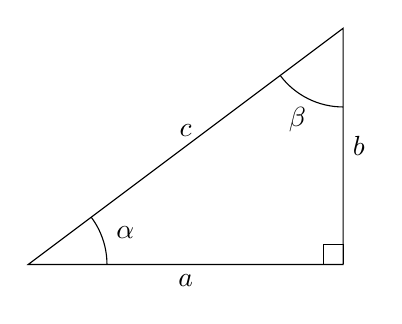
\begin{tikzpicture}
\draw (0,0) coordinate (o);
\draw (4,0) coordinate (u);
\draw (4,3) coordinate (v);
\draw (o)--(u) node[midway, below]{$a$}
--(v) node[midway, right]{$b$}
--(o) node[midway, above]{$c$} --cycle;
\tkzMarkRightAngle(o,u,v);
\tkzMarkAngle(o,v,u);
\tkzLabelAngle[pos=1.3](o,v,u){$\beta$};
\tkzMarkAngle(u,o,v);
\tkzLabelAngle[pos=1.3](u,o,v){$\alpha$};
\end{tikzpicture}

$$
c^2=a^2+b^2
$$

$$
\sin(\alpha)=\frac{b}{c},\quad
\cos(\alpha)=\frac{a}{c},\quad
\tan(\alpha)=\frac{b}{a},\quad
$$

$$
\alpha=\arcsin\frac{b}{c},\quad
=\arccos\frac{b}{c},\quad
=\arctan\frac{b}{c},\quad
$$

$$
\alpha=\textrm{Imag}(\ln(a+bi))\cdot\frac{180^\circ}{\pi}
$$

\end{document}